\section{DL8 Algorithm}
%\newcommand{\Proc}[1]{\textbf{Procedure #1}}
\begin{algorithm}
	\DontPrintSemicolon
	\caption{$DL8(maxdepth, minsup)$}
	\label{algo:1}
	\textbf{struct} $BestTree\{\ tree : Tree; error : float\ \}$\;
	$cache \gets HashSet < Itemset, BestTree >$\;
	$(\tau, b) \gets \verb|DL8-Recurse|(\emptyset)$\;
	\Return $\tau$\;
	\textbf{Procedure} \texttt{DL8-Recurse}$(I)$\;
		$solution \gets cache.get(I)$\;
		\If{solution was found}{
			\Return($solution.tree, solution.error$)\;
		}
		\If{$leaf\_error(I) = 0\ or\ |I| = maxdepth$}{
			\Return($make\_leaf(I), leaf\_error (I)$)\;
		}
		$(\tau, b) \gets (make\_leaf(I), leaf\_error (I))$\;
		\For{all attributes $i$}{
			\If{$|cover (I \cup \{i\})| \ge minsup$ and $|cover (I \cup \{\neg i\})| \ge minsup$}{
				$(\tau_1, e_1) \gets \texttt{DL8-Recurse}(I \cup \{i\})$\;
				\If{$e_1 \le b$}{
					$(\tau_2, e_2) \gets \texttt{DL8-Recurse}(I \cup \{i\})$\;
					\If{$e_1 + e_2 \le b$}{
						$(\tau, b) \gets (make\_tree(i, \tau_1, \tau_2), e_1 + e_2)$\;
					}
				}
			}
		}
		$cache.store(I, BestT ree(\tau, b))$\;
		\Return($\tau, b$)\;
\end{algorithm}

A high-level perspective of the DL8 algorithm is given in Algorithm \ref{algo:1}. Essentially, the algorithm recursively enumerates itemsets using the \verb|DL8-Recurse(I)| function. The post-condition of this function is that it returns the optimal decision tree for the transactions covered by itemset $I$, together with the quality of that tree. This optimal tree is calculated recursively using the observation that the best decision tree for a set of transactions can be obtained by considering all possible ways of partitioning the set of transactions into two, and determining the best tree for each partition recursively.

Figure \ref{fig:2} illustrates the search space of itemsets for the dataset of Table \ref{tab:1}, where all the possible itemsets are represented. Intuitively, DL8 starts at the top node of this search space, and calculates the optimal decision tree for the root based on its children.

A distinguishing feature of DL8 is its use of a cache. The idea behind this cache is to store the result of a call to \verb|DL8-Recurse(I)|. Doing so is effective as the same itemset can be reached by multiple paths in the search space: itemset $ab$ can be constructed by adding $b$ to itemset $a$, or by adding $a$ to itemset $b$. By storing the result, we can reuse the same result for both paths.

Note that the optimal decision tree for the root can only be calculated after all its children have been considered; hence, the algorithm will only produce a solution once the entire search space of itemsets has been considered.

In our pseudocode, we use the following other functions. Function $make\_leaf(I)$ returns a decision tree with one node, representing a leaf that predicts the majority class for the examples covered by I. The function $make\_tree(i, \tau_1, \tau_2)$ returns a tree with a test on attribute $i$, and subtrees $\tau_1$ and $\tau_1$.

The code illustrates a number of optimizations implemented in DL8:
\begin{description}
	\item[Maximum depth pruning] In line 9 the search is stopped as soon as the itemsets considered are too long;
	\item[Minimum support pruning] In line 13 an attribute is not considered if one of its branches has insufficient support ; in our running example, the itemset $\{a, b, c\}$ is not considered due to this optimization;
	\item[Purity pruning] In line 9 the search is stopped if the error for the current itemset is already 0;
	\item[Quality bounds] In the loop of lines 12–18, the best solution found among the children is maintained, and used to prune the second branch for an attribute if the first branch is already worse than the best solution found so far.
\end{description}
 
We omit a number of optimizations in this pseudo-code that can be found in the original publication, in particular, optimizations that concern the incremental maintenance of data structures. While we will use most of these optimizations in our implementation as well, we do not discuss thesein detail here for reasons of simplicity.

The most important optimization in DL8 that we do not use in this study is the \emph{closed itemset mining} optimization. The reason for this choice is that this optimization is hard to combine with a constraint on the depth of a decision tree. Similarly, while DL8 can be applied to other scoring functions than error, as long as the scoring function is \emph{additive}, we prioritize accuracy and the depth constraint here as we focus on solving the same problem as in recent MIP-based studies.
\begin{figure*}
	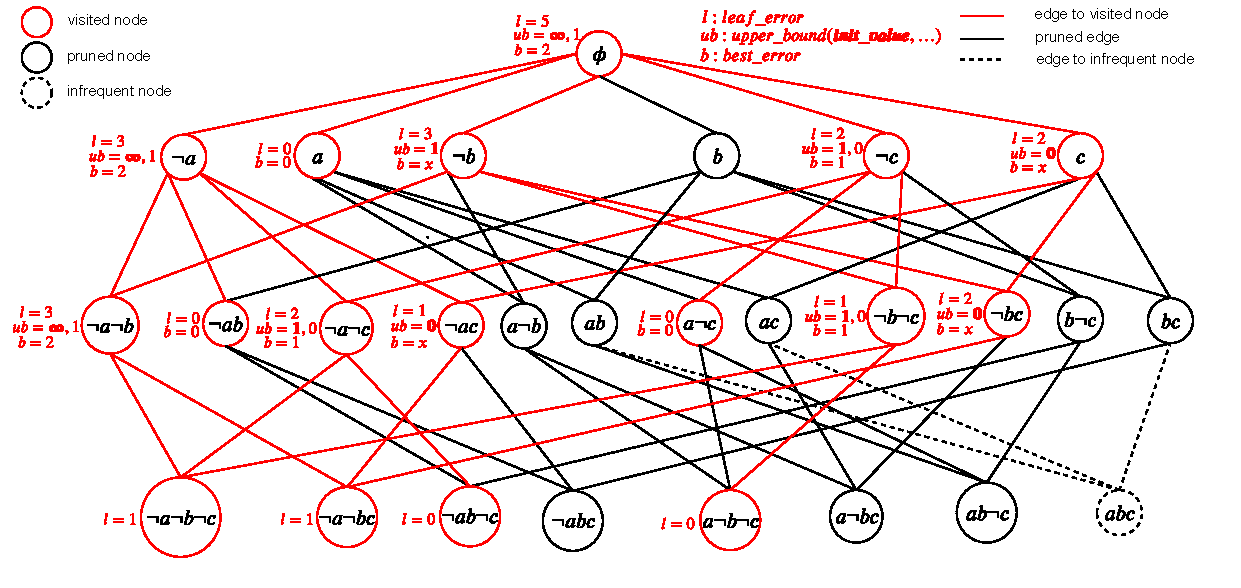
\includegraphics[width=\textwidth]{images/lattice_search}
	\caption{: Complete itemset lattice for introduction database and DL8.5 search execution}
	\label{fig:2}
\end{figure*}

